\chapter{Bildverarbeitung}
\section{Boxfilter}
Boxfilter
Faltung
$$ \widetilde{I}(i, j)=I \ast f =  \sum_{\alpha=-m}^m \sum_{\beta=-n}^n I(i-\alpha, j-\beta) \cdot f(\alpha, \beta)$$
Relevant: 
$$ \sum_{\alpha=-m}^m \sum_{\beta=-n}^n f(\alpha, \beta) \stackrel{!}{=} 1 $$
Boxfilter - Mittelwertfilter
$$ f=\frac{1}{9} \begin{bmatrix} 1&1&1 \\ 1&1&1 \\ 1&1&1 \end{bmatrix}$$
$$ \widetilde{I}(i, j)=\frac{1}{9} \sum_{\alpha=-1}^1 \sum_{\beta=-1}^1 I(i-\alpha, j-\beta) $$
Veranschaulicht wird dieses Vorgehen in \ref{fig:boxfilter}. Im linken Abschnitt ist das Originalbild mit einem gr\"o\ss{}eren Objekt und einigen St\"orpixeln zu sehen. Im rechten Abschnitt ist die gefilterte Version zu sehen: Die einzelnen St\"orpixel im oberen Abschnitt des Bildes sind deutlich abgeschw\"acht. Die Grenzen des Objektes in der rechten, unteren Ecke sind jedoch ebenso verschwommen. Bei mehrfacher Anwendung eines Mittelwertfilters konvergieren alle Pixelwerte gegen den Mittelwert der Pixel des gesamten Bildes. Der Mittelwertfilter ist somit ein Tiefpassfilter und sorgt anschaulich daf\"ur, dass Bilder verschwimmen.
\begin{figure}
 \centering
 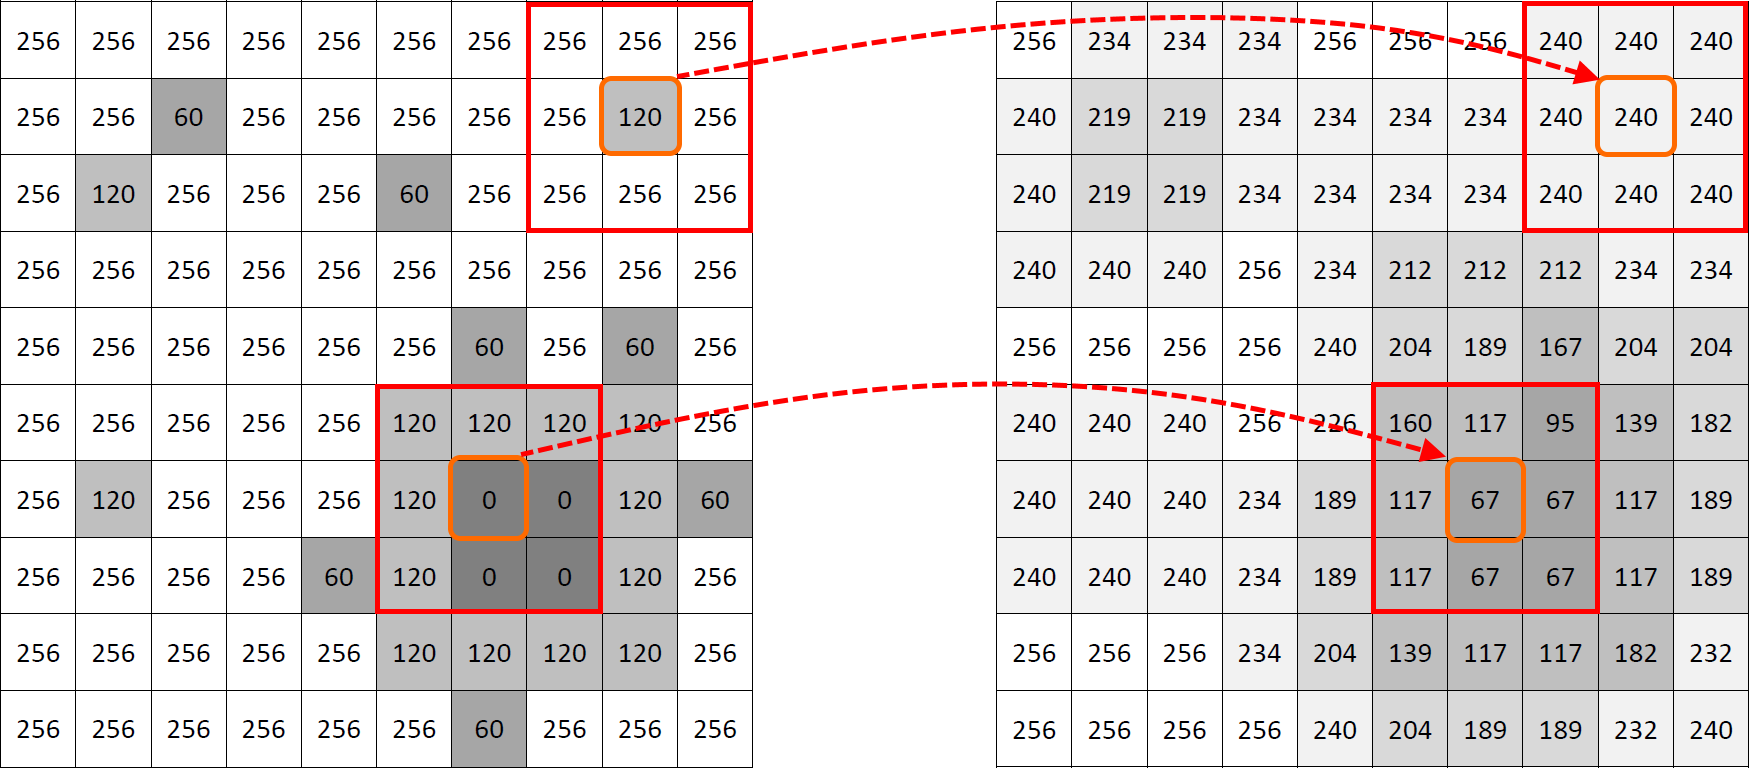
\includegraphics[width=1\textwidth]{media/filter/boxfilter_combined.png}
 \caption{Beispiel für 3x3 Boxfilter}
 \label{fig:boxfilter}
\end{figure}

Gau\ss{}filter:
\begin{equation}
 N(x, y) = \frac{1}{2\pi\sigma^2} e^{-\frac{x^2+y^2}{2\sigma^2}}
\end{equation}
Die Variable \( \sigma \) ergibt sich aus der Standardnormalverteilung mit \( \mu=0 \). Damit ergeben sich Filterkerne wie
\begin{multicols}{2}

\begin{equation*}
 G_{3x3}=\frac{1}{16} \begin{bmatrix} 1&2&1 \\ 2&4&2 \\ 1&2&1 \end{bmatrix}
\end{equation*}
 
 \columnbreak
 \begin{equation*}
 G_{5x5}=\frac{1}{256} \begin{bmatrix} 1&4&6&4&1 \\ 4&16&24&16&4 \\ 6&24&36&24&6 \\ 4&16&24&16&4 \\ 1&4&6&4&1 \end{bmatrix}
\end{equation*}
 
\end{multicols}



Sobelfilter zur Kantendetektion:
Analogie zentrale Differenz:
\begin{equation*}
 f^\prime (x)=\frac{f(x+\delta x)-f(x-\delta x)}{2\delta x}
\end{equation*}

\begin{multicols}{2}
\begin{align*}
 S_x &= \frac{1}{8} \begin{bmatrix}[r] -1&0&1 \\ -2&0&2 \\ -1&0&1 \end{bmatrix} \\
 S_u &= \frac{1}{8} \begin{bmatrix}[r] 0&-1&-2 \\ 1&0&-1 \\ 2&1&0 \end{bmatrix}
\end{align*}

\columnbreak

\begin{align*}
 S_y &= \frac{1}{8} \begin{bmatrix}[r] -1&-2&-1 \\ 0&0&0 \\ 1&2&1 \end{bmatrix} \\
 S_v &= \frac{1}{8} \begin{bmatrix}[r] -2&-1&0 \\ -1&0&1 \\ 0&1&2 \end{bmatrix}
\end{align*}
\end{multicols}

\section{Interpolation}

Interpolation: Suche 
\( f: \mathbb{R}^2\mapsto\mathbb{R}, f(x_n)=f_n, n=1,...,4 \)

Nearest-Neighbor-Interpolation:
\begin{equation*}
f: \mathbb{R}^2\mapsto\mathbb{R},f(x)=x_k,k=\underset{{l \in {1,..., 4}}}{arg\,min} (||x-x_l||)
\end{equation*}


Bilineare Interpolation:
\begin{eqnarray*}
 f: \mathbb{R}^2\mapsto\mathbb{R}, f(x, y)&=&\sum_{i=0}^1 \sum_{j=0}^1 a_{ij}x^iy^j \\
&=&a_{00}+a_{10}x+a_{01}y+a_{11}xy
\end{eqnarray*}

Bikubische Interpolation:
\begin{equation*}
 f: \mathbb{R}^2\mapsto\mathbb{R}, f(x, y)=\sum_{i=0}^3 \sum_{j=0}^3 a_{ij}x^iy^j
\end{equation*}

Die Parameter \(a_{ij} \) vorher analytisch berechnen.

\section{Morphologische Operationen}

